\section{Mathematical Model}

The testbed is a closed-loop simulation of vision-based rendezvous with a
tumbling, non-cooperative target, organised into four modules --- dynamics,
perception, estimation, and guidance-and-control --- so that each can be
validated in isolation and then exercised inside the complete loop
(Fig.~\ref{fig:system_architecture}). At every step the true states are
advanced, the target state is rendered into synthetic image measurements,
those are reduced to a relative pose, the pose is filtered into a navigation
state, and the resulting command acts on the chaser dynamics before the next
step. Perception errors therefore propagate into navigation and control, so
what is evaluated is the complete autonomous system rather than a set of
standalone algorithms.

\begin{figure}[t]
    \centering
    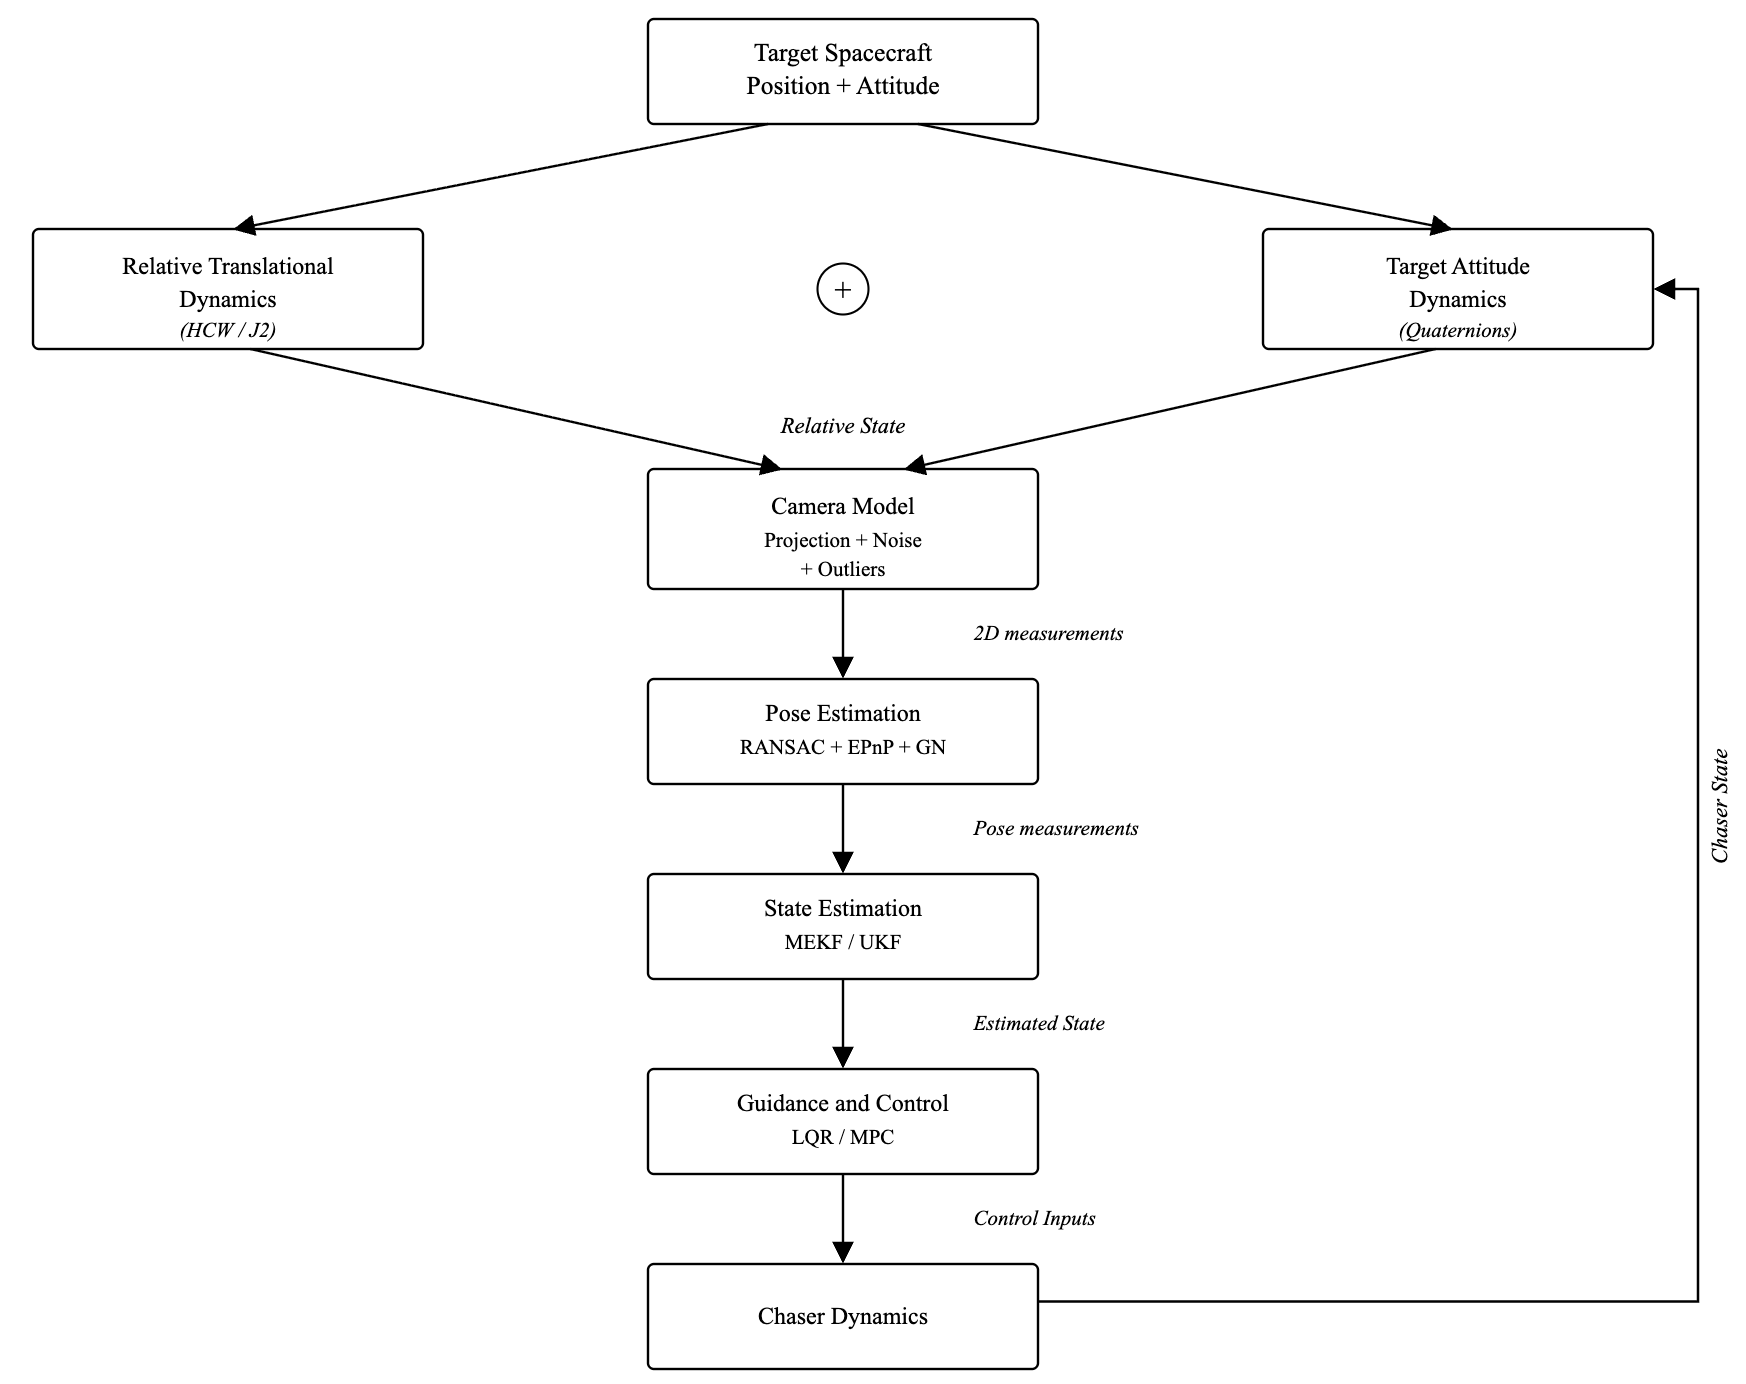
\includegraphics[width=\columnwidth]{figures/system_arch.png}
    \caption{Closed-loop architecture of the proposed vision-based
    autonomous spacecraft rendezvous framework.}
    \label{fig:system_architecture}
\end{figure}

\subsection{Reference Frames and Relative State}

Absolute quantities use the Earth Centred Inertial frame; the relative state
uses the target-centred Local Vertical Local Horizontal (LVLH) frame, with
radial axis $\hat{\mathbf{x}}$ from the Earth toward the target,
$\hat{\mathbf{z}}$ along the target orbital angular momentum and
$\hat{\mathbf{y}}=\hat{\mathbf{z}}\times\hat{\mathbf{x}}$. The translational
relative state is
$\mathbf{x}_{\mathrm{rel}}=[\mathbf{r}^{T}\ \mathbf{v}^{T}]^{T}$,
and the target attitude is carried as a unit quaternion $\mathbf{q}$ with
body-frame angular velocity $\boldsymbol{\omega}$, giving the attitude state
$\mathbf{x}_{\mathrm{att}}=[\mathbf{q}^{T}\ \boldsymbol{\omega}^{T}]^{T}$
subject to $\mathbf{q}^{T}\mathbf{q}=1$. The Hamilton convention is used
throughout; the dynamics and vision models store $\mathbf{q}$ scalar-first,
the estimator scalar-last as
$\mathbf{q}=[q_x\ q_y\ q_z\ q_w]^{T}$.

\subsection{Relative Orbital Dynamics}

For a near-circular reference orbit in LEO the relative translational
dynamics are the Hill--Clohessy--Wiltshire (HCW) equations
\cite{clohessy1960}. With mean motion $n=\sqrt{\mu/a^3}$, for gravitational
parameter $\mu$ and target semi-major axis $a$, the controlled equations are
\begin{equation}
\begin{aligned}
    \ddot{x} - 2n\dot{y} - 3n^2x &= f_x, \\
    \ddot{y} + 2n\dot{x} &= f_y, \\
    \ddot{z} + n^2z &= f_z,
\end{aligned}
\end{equation}
where $\mathbf{u}=[f_x\ f_y\ f_z]^{T}$ is the chaser control acceleration in
the LVLH frame. These assemble into the linear time-invariant form
$\dot{\mathbf{x}}_{\mathrm{rel}}
=\mathbf{A}_{\mathrm{HCW}}\mathbf{x}_{\mathrm{rel}}+\mathbf{B}\mathbf{u}$
with $\mathbf{B}=[\mathbf{0}_{3\times3}\ \ \mathbf{I}_{3}]^{T}$, whose
closed-form state transition is used by the guidance and control algorithms.
A higher-fidelity numerical path is retained for comparison, adding the
second-degree zonal harmonic $J_2$ to the two-body acceleration; it is not
exercised by any result reported here, where the unmodelled disturbance is
instead injected as a white acceleration on the true trajectory alone.

\subsection{Target Attitude Dynamics}

The target is a rigid body in potentially tumbling motion. Its quaternion
gives the direction cosine matrix $\mathbf{C}(\mathbf{q})$ from the target
body frame to the inertial frame, and the attitude evolves as
\begin{equation}
    \dot{\mathbf{q}}
    =
    \tfrac{1}{2}\mathbf{\Xi}(\mathbf{q})\boldsymbol{\omega},
    \qquad
    \mathbf{I}\dot{\boldsymbol{\omega}}
    =
    \boldsymbol{\tau}
    -\boldsymbol{\omega}\times(\mathbf{I}\boldsymbol{\omega}),
\end{equation}
with $\mathbf{\Xi}(\mathbf{q})$ the quaternion kinematic matrix, $\mathbf{I}$
the target inertia tensor and $\boldsymbol{\tau}$ the external body-frame
torque, zero in the scenarios considered here. Propagation uses an adaptive
high-order integrator with the quaternion renormalised each step. For
torque-free motion the rotational kinetic energy
$\tfrac{1}{2}\boldsymbol{\omega}^{T}\mathbf{I}\boldsymbol{\omega}$ and the
inertial angular momentum
$\mathbf{C}(\mathbf{q})\mathbf{I}\boldsymbol{\omega}$ are invariant, and are
monitored as numerical consistency checks.

\subsection{Camera Projection Model}

The perception module models a monocular camera on the chaser observing
fifteen analytically defined body-frame landmarks $\mathbf{P}_i^{b}$ on a
parametric Ariane 44L upper stage, distributed over the nose, mid-body ring
and nozzle, with the body-frame origin at the cylindrical centre and its
$x$-axis along the symmetry axis. The camera sits at the chaser with no
mounting rotation or lever arm, so the target attitude supplies the rotation
$\mathbf{R}_{bt}\in SO(3)$ and the HCW relative position $\mathbf{r}$ the
translation,
\begin{equation}
    \mathbf{P}_i^{c} = \mathbf{R}_{bt}\mathbf{P}_i^{b} + \mathbf{r}.
\end{equation}
Landmarks are mapped to the image by the pinhole model, which defines the
projection $\pi(\cdot)$,
\begin{equation}
    \mathbf{p}_i
    =
    \begin{bmatrix} u_i \\ v_i \end{bmatrix}
    =
    \begin{bmatrix}
        f_x X_i^c/Z_i^c + c_x \\ f_y Y_i^c/Z_i^c + c_y
    \end{bmatrix},
    \quad
    \tilde{\mathbf{p}}_i = \mathbf{p}_i + \boldsymbol{\eta}_i,
\end{equation}
for focal lengths $f_x,f_y$ and principal point $(c_x,c_y)$, with zero-mean
Gaussian pixel noise
$\boldsymbol{\eta}_i\sim\mathcal{N}(\mathbf{0},\sigma_{\mathrm{px}}^2\mathbf{I}_2)$
added independently to each landmark. The model supports the Brown--Conrady
radial and tangential distortion polynomial, disabled here with
$k_1=k_2=p_1=p_2=0$. A landmark is visible only when
$Z_i^c>0$ and $(u_i,v_i)$ falls inside the $W\times H$ image; the surviving
correspondences $\{\tilde{\mathbf{p}}_i \leftrightarrow
\mathbf{P}_i^b\}_{i=1}^{N}$ are the input to the pose-estimation stage.
Controlled correspondence outliers can also be injected to test that stage
under degraded observations. Camera and noise values are listed in
Table~\ref{tab:experimental_parameters}.

\subsection{Perspective-$n$-Point Pose Estimation}

Given $N$ correspondences, the pose-estimation stage recovers
$\mathbf{R}_{bt}\in SO(3)$ and $\mathbf{t}\in\mathbb{R}^{3}$ for which
$\mathbf{P}_i^c=\mathbf{R}_{bt}\mathbf{P}_i^b+\mathbf{t}$ reprojects
consistently onto the measured image points. The initial estimate uses the
Efficient Perspective-$n$-Point (EPnP) algorithm \cite{lepetit2009epnp},
which requires at least four correspondences, writes each landmark as an
affine combination of four virtual control points, and solves the resulting
homogeneous system $\mathbf{M}\mathbf{x}=\mathbf{0}$ through the null space
of $\mathbf{M}$ by singular value decomposition
(Section~\ref{sec:epnp_gn}). Among the candidate null-space solutions the one
with the lowest mean reprojection error satisfying the positive-depth
chirality constraint is selected, the landmark configuration reconstructed
from the barycentric coefficients, and the pose
$(\hat{\mathbf{R}}_{bt},\hat{\mathbf{t}})$ recovered by a rigid-body
absolute-orientation solution, whose quality is the reprojection error
\begin{equation}
    e_i^{\mathrm{rep}}
    =
    \left\|
    \tilde{\mathbf{p}}_i
    -
    \pi\left(\hat{\mathbf{R}}_{bt}\mathbf{P}_i^b+\hat{\mathbf{t}}\right)
    \right\|_2,
    \qquad
    \bar e_{\mathrm{rep}}
    =
    \frac{1}{N}\sum_{i=1}^{N} e_i^{\mathrm{rep}} .
\end{equation}
An optional nonlinear refinement of this cost is applied on top of the EPnP
solution; because a global rotation-vector parameterisation is singular at
$\theta=\pi$, it is formulated on the $SO(3)$ manifold
(Section~\ref{sec:pnp_manifold}) and is not used in the closed-loop pipeline.

\subsubsection{RANSAC-Based Outlier Rejection}

To tolerate incorrect correspondences the EPnP solver is wrapped in a RANSAC
stage \cite{fischler1981ransac} following the locally optimised strategy of
Chum and Matas~\cite{chum2003loransac}: a minimal subset is sampled, an EPnP
hypothesis generated, and correspondences with
$e_i^{\mathrm{rep}}<\tau_{\mathrm{rep}}$ counted as inliers. The largest
consensus set wins, with mean inlier reprojection error as the tie-break, and
the pose is refitted on its inliers. Sampling terminates adaptively once
\begin{equation}
    k \;\geq\; \frac{\log(1-p)}{\log\!\left(1-w^{s}\right)},
\end{equation}
where $w$ is the observed inlier ratio, $s$ the minimal sample size and $p$
the desired confidence level, subject to the iteration budget and inlier
threshold of Table~\ref{tab:experimental_parameters}.

\subsection{State Estimation}

Pose solutions are instantaneous and corrupted by image noise and pose-solver
error, so a recursive estimator supplies a temporally consistent relative
state. A Multiplicative Extended Kalman Filter (MEKF) \cite{markley2003} and
an error-state Unscented Kalman Filter (UKF) \cite{julier2004} are compared,
sharing nominal state, process and measurement models so that the filtering
formulation is the only difference. The nominal navigation state is
\begin{equation}
    \mathbf{x}
    =
    \begin{bmatrix}
        \mathbf{r}^{T} & \mathbf{v}^{T} &
        \mathbf{q}^{T} & \boldsymbol{\omega}^{T}
    \end{bmatrix}^{T},
    \quad
    \delta\mathbf{x}
    =
    \begin{bmatrix}
        \delta\mathbf{r}^{T} & \delta\mathbf{v}^{T} &
        \delta\boldsymbol{\alpha}^{T} & \delta\boldsymbol{\omega}^{T}
    \end{bmatrix}^{T},
\end{equation}
with $\|\mathbf{q}\|=1$. Because additive quaternion perturbations violate
that constraint, the covariance is carried in the 12-dimensional error state,
$\delta\boldsymbol{\alpha}$ being the small-angle attitude error. The nominal
state is propagated through the nonlinear dynamics and the covariance through
the error-state transition matrix $\mathbf{F}_k$,
\begin{equation}
    \mathbf{x}_{k+1}^{-} = f(\mathbf{x}_{k}^{+},\Delta t),
    \qquad
    \mathbf{P}_{k+1}^{-}
    =
    \mathbf{F}_{k}\mathbf{P}_{k}^{+}\mathbf{F}_{k}^{T}+\mathbf{Q}_{k},
\end{equation}
where $\Delta t$ is the sampling interval and $\mathbf{Q}_k$ is
acceleration-driven as derived in Section~\ref{sec:process_noise}.

The measurement supplied to the estimator is a relative translation and a
target attitude. In the filter-isolation experiment it is generated directly
from the true state with additive Gaussian noise,
\begin{equation}
    \mathbf{z}_{k}
    =
    \begin{bmatrix}
        \mathbf{r}_{k}^{\mathrm{true}}\\
        \boldsymbol{\rho}_{k}^{\mathrm{true}}
    \end{bmatrix}
    +
    \begin{bmatrix}
        \boldsymbol{\nu}_{r,k}\\ \boldsymbol{\nu}_{\rho,k}
    \end{bmatrix},
    \qquad
    \mathbf{R}
    =
    \begin{bmatrix}
        \sigma_{\mathrm{pos}}^{2}\mathbf{I}_{3} & \mathbf{0}\\
        \mathbf{0} & \sigma_{\mathrm{att}}^{2}\mathbf{I}_{3}
    \end{bmatrix},
\end{equation}
where $\boldsymbol{\rho}$ is the rotation vector of the target attitude and
the noise standard deviations are those of
Table~\ref{tab:experimental_parameters}. The complete vision-to-estimation
pipeline is evaluated separately in Section~\ref{sec:results}.

\subsubsection{Multiplicative Extended Kalman Filter}

With predicted measurement $\hat{\mathbf{z}}_{k}=h(\mathbf{x}_{k}^{-})$,
innovation $\mathbf{y}_{k}=\mathbf{z}_{k}-\hat{\mathbf{z}}_{k}$ and
innovation covariance $\mathbf{S}_{k}=\mathbf{H}_{k}\mathbf{P}_{k}^{-}
\mathbf{H}_{k}^{T}+\mathbf{R}_{k}$, the gain and error-state correction are
$\mathbf{K}_{k}=\mathbf{P}_{k}^{-}\mathbf{H}_{k}^{T}\mathbf{S}_{k}^{-1}$ and
$\delta\mathbf{x}_{k}=\mathbf{K}_{k}\mathbf{y}_{k}$, the attitude component of $\mathbf{y}_k$ being formed multiplicatively on
$SO(3)$, which makes $\mathbf{H}_k$ exact and constant
(Section~\ref{sec:mekf_residual}). Translational and angular-velocity
corrections are applied additively, while the attitude correction is applied
multiplicatively to the nominal attitude,
\begin{equation}
    \mathbf{q}_{k}^{+}
    =
    \operatorname{norm}
    \left(
        \operatorname{Exp}(\delta\boldsymbol{\alpha}_{k})
        \otimes
        \mathbf{q}_{k}^{-}
    \right),
\end{equation}
and the covariance is updated in Joseph form,
\begin{equation}
    \mathbf{P}_{k}^{+}
    =
    (\mathbf{I}-\mathbf{K}_{k}\mathbf{H}_{k})
    \mathbf{P}_{k}^{-}
    (\mathbf{I}-\mathbf{K}_{k}\mathbf{H}_{k})^{T}
    +
    \mathbf{K}_{k}\mathbf{R}_{k}\mathbf{K}_{k}^{T},
\end{equation}
symmetrised after prediction and update. Measurements statistically
inconsistent with the prediction are rejected by a Mahalanobis gate on the
squared normalised innovation,
$d_k^2=\mathbf{y}_{k}^{T}\mathbf{S}_{k}^{-1}\mathbf{y}_{k}\leq\gamma$, with
$\gamma$ the chi-square threshold of
Table~\ref{tab:experimental_parameters}; a failing measurement is discarded
and the predicted state retained. The attitude part of the innovation is
expressed as a principal rotation vector before the distance is evaluated.

\subsubsection{Unscented Kalman Filter}

The UKF replaces the analytic linearisation by propagating sigma points
through the nonlinear models, using the same 12-dimensional error state. For
$n_x=12$ the scaled unscented transform sets
\begin{equation}
    \lambda = \alpha^2(n_x+\kappa)-n_x,
    \qquad
    W_0^{(m)} = \frac{\lambda}{n_x+\lambda},
\end{equation}
so that both the sigma-point spread and the centre weight are controlled by
$\alpha$; the sigma points and the remaining weights
follow the standard scaled transform \cite{julier2004}. Each error-state sigma
point is applied to the nominal state --- attitude perturbations
multiplicatively, preserving the unit-norm constraint --- and propagated
through the relative translational and attitude dynamics, giving the
cross-covariance $\mathbf{P}_{xz}$ and the innovation covariance
$\mathbf{P}_{zz}$, from which
$\mathbf{K}=\mathbf{P}_{xz}\mathbf{P}_{zz}^{-1}$ and
$\delta\mathbf{x}=\mathbf{K}(\mathbf{z}-\hat{\mathbf{z}})$, the attitude
correction again applied multiplicatively. The implemented filter uses
$\alpha=0.5$, $\beta=2$ and $\kappa=0$.

\subsection{Guidance and Control}

The guidance-and-control module drives the chaser with either a Linear
Quadratic Regulator (LQR) or a receding-horizon Model Predictive Controller
(MPC), both acting on the HCW relative dynamics. The MPC imposes an explicit
thrust constraint and, during the terminal phase, an approach-cone constraint
formulated as a softened second-order cone (Section~\ref{sec:cone}). The
commanded acceleration $\mathbf{u}$ updates the chaser state and produces the
next camera observation, closing the perception--navigation--control loop.

\subsection{Refinement of the EPnP Control-Point Coefficients}
\label{sec:epnp_gn}

Writing the $N$ world points as affine combinations of control points,
$\mathbf{P}_i = \sum_{j} \alpha_{ij}\,\mathbf{c}_j$ with
$\sum_j \alpha_{ij} = 1$, the projection equations stack into
$\mathbf{M}\mathbf{x} = \mathbf{0}$, where $\mathbf{x}$ collects the control
points in the camera frame. The solution lies in the null space of
$\mathbf{M}$,
\begin{equation}
\mathbf{x} = \sum_{k=1}^{n} \beta_k \mathbf{v}_k ,
\label{eq:epnp_null}
\end{equation}
and the coefficients $\beta_k$ are fixed by requiring that the
inter-control-point distances be preserved:
\begin{equation}
\bigl\| \textstyle\sum_k \beta_k (\mathbf{v}_k^{[i]} - \mathbf{v}_k^{[j]}) \bigr\|^2
= \| \mathbf{c}_i - \mathbf{c}_j \|^2 ,
\qquad i < j .
\label{eq:epnp_dist}
\end{equation}

Equation~\eqref{eq:epnp_dist} is quadratic in $\boldsymbol{\beta}$.
Linearising in the products $b_{kl} = \beta_k \beta_l$ gives a linear system
$\mathbf{L}\mathbf{b} = \boldsymbol{\rho}$ whose least-squares solution yields
an initial $\boldsymbol{\beta}$ by relinearisation,
$\beta_1 = \sqrt{|b_{11}|}$ and $\beta_k = b_{1k}/\beta_1$. This is an
\emph{initialisation}, not the answer, and treating it as the answer costs
roughly a factor of four in accuracy (Sec.~\ref{sec:res_pose}). We refine
$\boldsymbol{\beta}$ by Gauss--Newton directly on \eqref{eq:epnp_dist}. With
$\mathbf{D}_{ij}$ the matrix whose $k$-th column is
$\mathbf{v}_k^{[i]} - \mathbf{v}_k^{[j]}$ and
$\mathbf{d}_{ij} = \mathbf{D}_{ij}\boldsymbol{\beta}$, the residual and its
Jacobian are
\begin{align}
f_{ij}(\boldsymbol{\beta}) &= \mathbf{d}_{ij}^{\top}\mathbf{d}_{ij}
                              - \|\mathbf{c}_i - \mathbf{c}_j\|^2 ,
\label{eq:epnp_resid}\\
\frac{\partial f_{ij}}{\partial \beta_m}
  &= 2\, \mathbf{d}_{ij}^{\top} \mathbf{D}_{ij}\,\mathbf{e}_m .
\label{eq:epnp_jac}
\end{align}
Ten iterations of $\boldsymbol{\beta} \leftarrow \boldsymbol{\beta} +
\boldsymbol{\delta}$, with $\boldsymbol{\delta}$ the least-squares solution of
$\mathbf{J}\boldsymbol{\delta} = -\mathbf{f}$, suffice in every case tested.

\paragraph{The coplanar case.}
The control points are the centroid plus the principal axes of the point
cloud, scaled by the corresponding singular values. When the cloud is
coplanar the third singular value vanishes, so a fourth control point
coincides with the centroid, the barycentric system becomes singular, and
three columns of $\mathbf{M}$ vanish identically --- giving $\mathbf{M}$ a
four-dimensional null space for algebraic rather than geometric reasons. The
planar configuration must therefore be detected, from $s_3 / s_1 < \epsilon$,
and parameterised with \emph{three} control points, so that
$\mathbf{x} \in \mathbb{R}^{9}$ and $\mathbf{M}$ is $2N \times 9$.
Approximately 3\% of random six-point subsets of the target's keypoint set
are exactly coplanar, so this is not an edge case.

\subsection{Pose Refinement on the $SO(3)$ Manifold}
\label{sec:pnp_manifold}

The refinement stage minimises the reprojection cost
\begin{equation}
E(\mathbf{R}, \mathbf{t}) = \sum_{i} w_i \,
\bigl\| \tilde{\mathbf{p}}_i - \pi(\mathbf{R}\mathbf{P}_i + \mathbf{t}) \bigr\|^2 .
\label{eq:lm_cost}
\end{equation}
Parameterising $\mathbf{R} = \exp([\mathbf{r}]_\times)$ by a \emph{global}
rotation vector is convenient but singular at $\|\mathbf{r}\| = \pi$, where the
derivative of the exponential map is unbounded --- not a remote possibility
here, since a camera whose boresight is aligned with a world axis produces
$\operatorname{tr}(\mathbf{R}) = -1$ exactly, i.e.\ $\theta = \pi$, and such
poses are the natural fixtures for an on-axis approach. We therefore carry
$\mathbf{R}$ as a matrix and optimise over a local increment. Using a
left-multiplicative update,
\begin{equation}
\mathbf{R} \leftarrow \exp([\boldsymbol{\delta\omega}]_\times)\,\mathbf{R},
\qquad
\mathbf{t} \leftarrow \mathbf{t} + \boldsymbol{\delta t} ,
\label{eq:lm_update}
\end{equation}
and noting that $\exp([\boldsymbol{\delta}]_\times)\mathbf{v} \approx
\mathbf{v} - [\mathbf{v}]_\times \boldsymbol{\delta}$, the Jacobian blocks at
$\boldsymbol{\delta} = \mathbf{0}$ are
\begin{equation}
\frac{\partial \mathbf{P}^c_i}{\partial \boldsymbol{\delta\omega}}
  = -[\mathbf{R}\mathbf{P}_i]_\times ,
\qquad
\frac{\partial \mathbf{P}^c_i}{\partial \boldsymbol{\delta t}} = \mathbf{I}_3 ,
\label{eq:lm_jac}
\end{equation}
so that with the perspective Jacobian
\begin{equation}
\frac{\partial \pi}{\partial \mathbf{P}^c}
= \begin{bmatrix}
f_x / Z & 0 & -f_x X / Z^2 \\
0 & f_y / Z & -f_y Y / Z^2
\end{bmatrix}
\label{eq:proj_jac}
\end{equation}
the stacked Jacobian is
$\mathbf{J}_i = (\partial \pi / \partial \mathbf{P}^c)\,
[-[\mathbf{R}\mathbf{P}_i]_\times \;\; \mathbf{I}_3]$.
Because $\boldsymbol{\delta\omega}$ is always near zero, the local
parameterisation is well conditioned wherever the optimiser is, and the
singularity cannot be reached. Two further conditions keep the iteration
honest. The residual and the Jacobian must be evaluated at the same point ---
clamping $Z$ in one and not the other lets Levenberg--Marquardt accept steps
that lower a cost it is not actually computing, and the translation then
diverges without bound while the reported cost stays finite. And chirality
must be enforced: any pose placing a weighted point at or behind the camera
plane is assigned infinite cost and rejected, so failure is visible rather
than silent.

\subsection{Multiplicative Attitude Residual}
\label{sec:mekf_residual}

Position enters the residual as a difference in the usual way; attitude
cannot, and the reason is worth setting out because the naive form is
superficially reasonable. With $\hat{\mathbf{q}}$ the filter's estimate,
encoding both attitudes as global rotation vectors and subtracting,
$\boldsymbol{\nu}_{att} = \log(\mathbf{q}_{meas}) - \log(\hat{\mathbf{q}})$,
fails at $\theta = \pi$: two attitudes separated by an arbitrarily small
rotation, one either side of $\pi$, map to nearly antipodal rotation vectors,
so a vanishing attitude error produces a residual of magnitude $2\pi$. The
linearised residual is then meaningless, and the Jacobian condition number
grows without bound as $\theta \to \pi$. The residual must instead be formed
on the group and expressed in the tangent space at the estimate,
\begin{equation}
\boldsymbol{\delta\alpha}
  = \log\!\bigl( \mathbf{q}_{meas} \otimes \hat{\mathbf{q}}^{-1} \bigr) ,
\label{eq:att_residual}
\end{equation}
where $\log(\cdot)$ returns the rotation vector of its argument and the sign of
the relative quaternion is chosen so that its scalar part is non-negative,
selecting the short rotation. This is exact for every attitude, and it has a
second benefit. Because the error state is defined by the same
left-multiplicative perturbation,
$\mathbf{q} = \exp(\tfrac{1}{2}\boldsymbol{\delta\alpha}) \otimes
\hat{\mathbf{q}}$, the residual \emph{is} the attitude error state to first
order, and the measurement Jacobian becomes exact and constant:
\begin{equation}
\mathbf{H} =
\begin{bmatrix}
\mathbf{I}_3 & \mathbf{0} & \mathbf{0} & \mathbf{0} \\
\mathbf{0} & \mathbf{0} & \mathbf{I}_3 & \mathbf{0}
\end{bmatrix} .
\label{eq:H_exact}
\end{equation}
No finite differencing is required, and $\mathbf{R}_{att} = \sigma_{att}^2
\mathbf{I}_3$ becomes a genuine tangent-space covariance rather than an
approximation. The measurement noise must be injected on the same side for
this to hold: a physical attitude perturbation is
$\mathbf{q}_{meas} = \exp(\tfrac{1}{2}\boldsymbol{\eta}) \otimes \mathbf{q}$
with $\boldsymbol{\eta} \sim \mathcal{N}(\mathbf{0},
\sigma_{att}^2\mathbf{I}_3)$.

\subsection{Acceleration-Driven Process Noise}
\label{sec:process_noise}

The dominant unmodelled effects on the relative translation --- differential
$J_2$, differential drag, thruster execution error --- act as an
\emph{acceleration}, so the process noise must drive position and velocity
jointly. Treating the disturbance as white acceleration of density
$\sigma_a$ over a step $\Delta t$ gives the standard kinematic block
\begin{equation}
\begin{bmatrix}
\mathbf{Q}_{rr} & \mathbf{Q}_{rv} \\
\mathbf{Q}_{vr} & \mathbf{Q}_{vv}
\end{bmatrix}
= \sigma_a^2
\begin{bmatrix}
\tfrac{1}{3}\Delta t^3 \mathbf{I}_3 & \tfrac{1}{2}\Delta t^2 \mathbf{I}_3 \\
\tfrac{1}{2}\Delta t^2 \mathbf{I}_3 & \Delta t\, \mathbf{I}_3
\end{bmatrix},
\label{eq:Q_kin}
\end{equation}
with the same structure on the attitude and rate block for an angular
acceleration density. The off-diagonal terms are not optional: position and
velocity errors driven by a common acceleration are correlated, and a diagonal
$\mathbf{Q}$ asserts that they are not, which weakens the information a
position measurement carries about velocity. A diagonal alternative that
models position as an independent random walk is worse still --- a position
noise of $0.05$~m per step contributes
$\mathbf{Q}_{rr} = 2.5 \times 10^{-3}$~m$^2$, roughly three hundred times the
$8.3 \times 10^{-6}$~m$^2$ that a physically plausible
$5 \times 10^{-4}$~m/s$^2$ disturbance produces over a one-second step. The
filter is then needlessly conservative, and its $\mathbf{Q}$ describes a
disturbance that is not present in the truth, so the consistency statistics of
Eq.~\eqref{eq:nis} become uninformative.

\subsection{Approach Corridor as a Second-Order Cone}
\label{sec:cone}

The terminal approach is confined to a cone of half-angle $\theta_c$ about the
$+x$ (radial) approach axis. For a predicted position
$\mathbf{r}_k = [x_k,\ y_k,\ z_k]^{\top}$ the constraint is
\begin{equation}
\sqrt{y_k^2 + z_k^2} \;\le\; x_k \tan\theta_c ,
\qquad k = 0,\dots,N-1 .
\label{eq:cone}
\end{equation}
Three properties of \eqref{eq:cone} matter and are each easy to lose. It is a
\emph{cone}, not a wedge: both transverse components appear, and constraining
$|y_k|$ alone leaves the cross-track axis free. It is \emph{signed}: the
right-hand side must be non-negative, so \eqref{eq:cone} implies
$x_k \ge 0$, whereas replacing $x_k$ by $|x_k|$ mirrors the corridor into
$x < 0$ and is satisfied by a chaser sitting behind the target. And the
constrained quantity is the predicted state
$\mathbf{X}(\mathbf{U}) = \mathbf{S}_x \mathbf{e} + \mathbf{S}_u \mathbf{U}$;
evaluating the radius on the free response $\mathbf{S}_x\mathbf{e}$ makes the
right-hand side independent of the decision variable, and the constraint
ceases to constrain anything. Written for a nonlinear-programming solver,
\eqref{eq:cone} becomes
$g_k(\mathbf{U}) \ge 0$ with
\begin{equation}
g_k(\mathbf{U}) = \tan\theta_c \; x_k(\mathbf{U})
   - \sqrt{y_k(\mathbf{U})^2 + z_k(\mathbf{U})^2 + \varepsilon^2},
\label{eq:cone_g}
\end{equation}
where $\varepsilon$ (here $10^{-6}$~m) keeps $g_k$ differentiable on the axis
at the cost of a marginally conservative constraint. The gradient is
\begin{equation}
\nabla_{\mathbf{U}} g_k = \tan\theta_c \, \mathbf{S}_u^{x,k}
 - \frac{y_k \mathbf{S}_u^{y,k} + z_k \mathbf{S}_u^{z,k}}
        {\sqrt{y_k^2 + z_k^2 + \varepsilon^2}} ,
\label{eq:cone_grad}
\end{equation}
with $\mathbf{S}_u^{x,k}$ the row of $\mathbf{S}_u$ selecting $x_k$.

Imposed as a hard constraint, \eqref{eq:cone} destroys recursive feasibility:
once the chaser lies outside the cone there may be no admissible input
returning the first predicted state to it, and the quadratic program is
infeasible. Since an infeasible solve is what produces a silent zero-thrust
command, we soften the corridor with slack $s_k \ge 0$ under a linear penalty,
\begin{equation}
\min_{\mathbf{U},\,\mathbf{s}} \;
\tfrac{1}{2}\mathbf{U}^{\top}\mathbf{H}\mathbf{U} + \mathbf{f}^{\top}\mathbf{U}
+ \rho \sum_{k} s_k
\quad \text{s.t.} \quad g_k(\mathbf{U}) + s_k \ge 0 ,
\label{eq:cone_soft}
\end{equation}
which is always feasible and drives $s_k \to 0$ whenever the hard constraint
can be met. The corridor solve is judged on the quantity it exists to reduce,
$\sum_k \max(0, -g_k)$, rather than on the solver's own convergence flag, and
is attempted only when the box-constrained optimum already violates
\eqref{eq:cone} --- an active-set shortcut that leaves the solution unchanged
when the corridor is inactive and reduces the per-step cost by two orders of
magnitude.
